\documentclass[Serif, 10pt, brown]{beamer}
\usepackage{booktabs,xcolor}
\usepackage{pifont}
\newcommand*\CHECK{\ding{51}}
\usepackage{array}
\newcolumntype{P}[1]{>{\centering\arraybackslash}p{#1}}

\usepackage{setspace,mathtools,amssymb,multirow,array,amsmath,tikz}
\usepackage[normalsize]{subfigure}
\usetikzlibrary{patterns,automata,positioning,decorations.pathreplacing,decorations}
\usepackage{curves}
\usepackage{caption}
\usepackage{wasysym}
\usepackage{epsfig,epstopdf,graphicx}

\curvewarnfalse

\newtheorem{proposition}{Proposition}
\theoremstyle{example}
\newtheorem{theoremh}{Theorem}
\theoremstyle{plain}
\renewcommand{\textfraction}{0.01}
\renewcommand{\floatpagefraction}{0.99}
\newcommand{\ul}{\underline}
\newcounter{units}
\setbeamercovered{dynamic}
\logo{
\includegraphics[width=0.5in,keepaspectratio]{iitb_logo.png}}

\mode<presentation>{
    \usetheme[right,currentsection,hideothersubsections]{UTD}
    \useoutertheme{sidebar}
    \useinnertheme[shadow]{rounded}
    \usecolortheme{whale}
    \usecolortheme{orchid}
    \usefonttheme[onlymath]{serif}
    \setbeamertemplate{footline}{\centerline{Slide \insertframenumber/\inserttotalframenumber}}
}

\usebeamercolor[fg]{author in sidebar}
\title[{Systems for LLMs}]{\sc Benchmarking and Performance Analysis of LLM Inferencing Systems}
\author[\ul{Authors}]{{\textbf{Saksham Rathi}}}
\institute[UTD]{\sc\small Systems for LLMs\\ Under Prof. Mythili Vutukuru}
\date[UCI]{Indian Institute of Technology Bombay \\ Autumn 2025-26}

\begin{document}
\frame{\titlepage}

\begin{frame}{Contents}
	\tableofcontents
\end{frame}

% =========================================================
\section{Workload Picked}

% --- NEW: Split into two slides ---
\begin{frame}{Workload Setup}
\begin{itemize}
    \item \textbf{Goal:} Evaluate inference performance of LLMs under short queries with large shared context.
    \item \textbf{Model:} Qwen 0.5B, Tiny Llama 1.1B, served using vLLM/SGLang/Transformers.
    \item \textbf{Hardware:} NVIDIA RTX6000 48GB GPU.
    \item \textbf{Metrics:} Throughput (req/s), latency, GPU utilization.
\end{itemize}

\begin{table}[h!]
\centering
\scriptsize
\begin{tabular}{|l|c|}
\hline
\textbf{Parameter} & \textbf{Value/Range} \\
\hline
System Prompt Length & $\approx$1500 tokens (shared across requests) \\
Query Rate & 5–700 req/sec \\
Query Length & 10–20 tokens \\
Output Length & 30–50 tokens \\
Batch Size & Adaptive \\
\hline
\end{tabular}
\caption{Workload Characteristics}
\end{table}
\end{frame}


\section{Batch of Requests through Various Engines}

% --- NEW setup slide ---
\begin{frame}{Experiment Setup: Engine Comparison}
\begin{itemize}
    \item Compare inference engines: \textbf{Transformers}, \textbf{vLLM}, \textbf{SGLang}, \textbf{NEO}.
    \item Batch of 24 requests, each sharing the same system prompt.
    \item Each request: $\sim$20 input tokens $\rightarrow$ $\sim$40 generated tokens.
    \item Measure \textbf{total time taken} to process the batch.
\end{itemize}

\begin{block}{Hypothesis}
Engines leveraging prefix caching (e.g., SGLang) should perform far better than naive batching in Transformers.
\end{block}
\end{frame}

\begin{frame}{Batch of requests through various Engines}
    \begin{columns}[T, totalwidth=\textwidth]
        \begin{column}{0.4\textwidth}
            \centering
            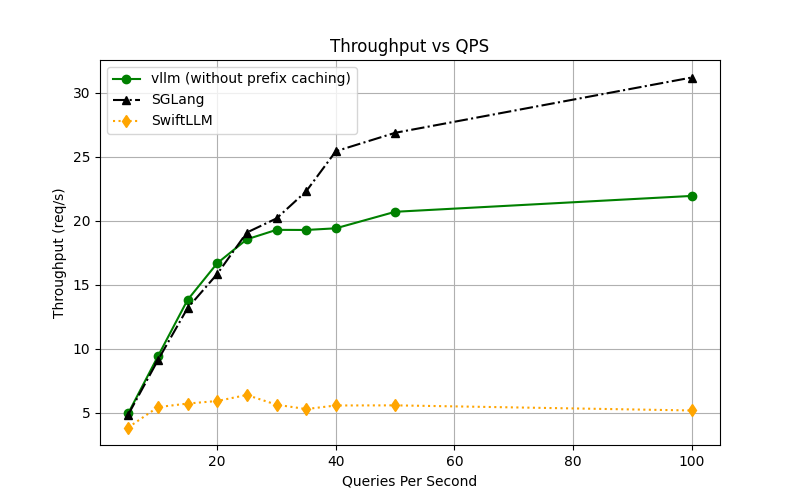
\includegraphics[width=\textwidth]{../results/throughput_vs_qps.png}
            \vspace{0.3em}
            \captionof{figure}{Throughput comparison across varying workloads}
        \end{column}
        \begin{column}{0.6\textwidth}
            \begin{itemize}
                \item \textbf{SwiftLLM:} lightweight vLLM clone (~2000 LOC), but performs the worst.
                \item \textbf{SGLang:} achieves best performance via radix-tree prefix sharing.
            \end{itemize}
            \begin{table}[h]
            \centering
            \scriptsize
            \begin{tabular}{|l|c|}
            \hline
            \textbf{Technique Used} & \textbf{Time (s)} \\
            \hline
            Transformers (batch = 1) & 30.21 \\
            Transformers (batch = 2) & 19.51 \\
            Transformers (batch = 3) & 18.64 \\
            vLLM (no system prompt pre-filling) & 0.45 \\
            SGLang (fork) & 1.03 \\
            SGLang (run\_batch) & 0.40 \\
            NEO & 0.55 \\
            \hline
            \end{tabular}
            \caption{Measuring the time taken to process a batch of 24 requests using different techniques}
            \end{table}
    
        \end{column}
    \end{columns}
\end{frame}


\section{LLM Request Timelines}

\begin{frame}{Experiment Setup: Request Timelines}
\begin{itemize}
    \item Aim: Measure time spent in \textbf{prefill} vs \textbf{decode} stages for 20 req/sec workload (sending a new request after every 0.05 seconds).
    \item Using vLLM V0 engine without chunked prefill.
    \item Tool: Custom logging of per-request timestamps.
\end{itemize}
\begin{figure}[h!]
\centering
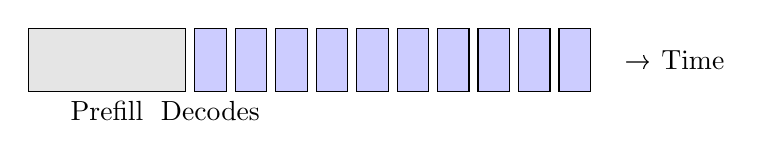
\begin{tikzpicture}[node distance=0.1cm]
\tikzstyle{block}=[draw,fill=gray!20,minimum height=0.8cm]
\def\prefillwidth{2cm}
\def\decodewidth{0.4cm}
\node[block,minimum width=\prefillwidth,label=below:{Prefill}] (p) {};

\foreach \i in {1,...,10} {
  \pgfmathtruncatemacro{\prev}{\i - 1}
  \ifnum\i=1
    \node[block,fill=blue!20,minimum width=\decodewidth,
          right=of p,label=below:{Decodes}] (d\i) {};
  \else
    \node[block,fill=blue!20,minimum width=\decodewidth,
          right=of d\prev,label=below:{}] (d\i) {};
  \fi
}
\node[right=of d10,xshift=0.2cm] {→ Time};

\end{tikzpicture}
\caption{Simplified per-request timeline}
\end{figure}
\end{frame}

\begin{frame}{Results: LLM Request Timelines}
\begin{columns}[T, totalwidth=\textwidth]
    \begin{column}{0.6\textwidth}
        \centering
        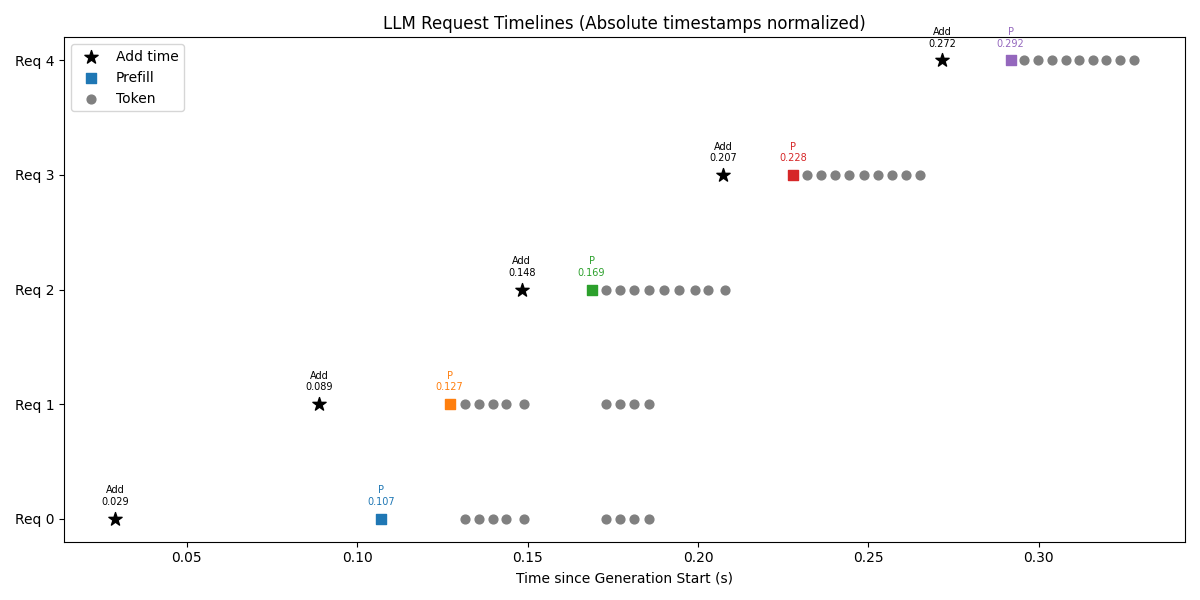
\includegraphics[width=\textwidth]{figures/llm_timelines_20.png}
        \captionof{figure}{20 Requests/sec – No chunked prefill – vLLM V0}
    \end{column}
    \begin{column}{0.4\textwidth}
        \begin{itemize}
            \item Prefill dominates runtime due to large prompt.
            \item Prefill and decode cannot overlap here.
            \item Low TTFT but high total latency.
        \end{itemize}
    \end{column}
\end{columns}
\end{frame}

\section{NSYS Measurements}

\begin{frame}{Results: NSYS Measurements}
\begin{block}{Goal}
Understand compute vs memory utilization and bottlenecks.
\end{block}
\vspace{1cm}
\centering
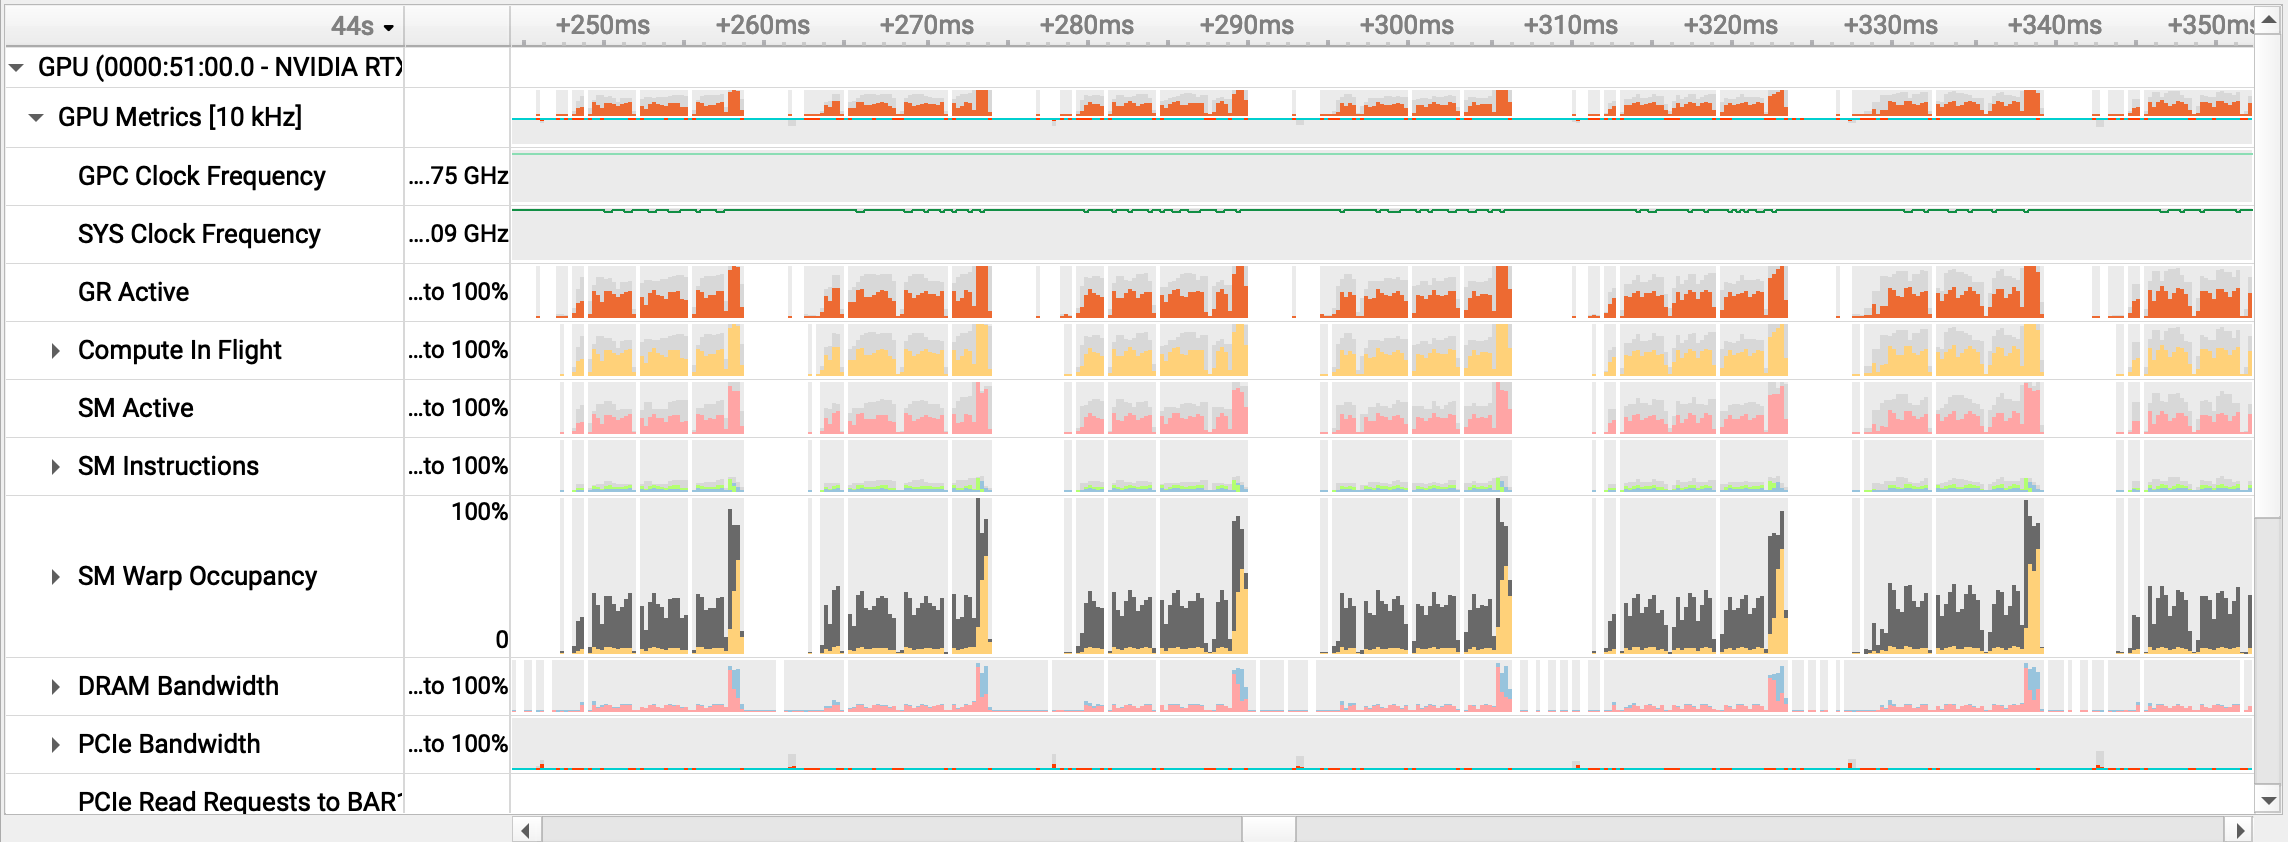
\includegraphics[width=\textwidth]{../results/nsys_metrics_llm_inference.png}
\captionof{figure}{NSYS Metrics Snapshot}
\end{frame}

\begin{frame}{Observation: NSYS Profiling}
\begin{itemize}
    \item Compute: SM Active and Warp occupancy.
    \item Memory: vLLM books full GPU memory upfront.
    \item vLLM scheduler stats show the actual KV Cache Usage.
    \item PCIe Bandwidth low → small workloads, minimal CPU transfer.
\end{itemize}
\end{frame}

\section{Throughput vs Load for vLLM}

\begin{frame}{Results: Throughput vs Load for vLLM}
\begin{columns}[T, totalwidth=\textwidth]
    \begin{column}{0.6\textwidth}
        \centering
        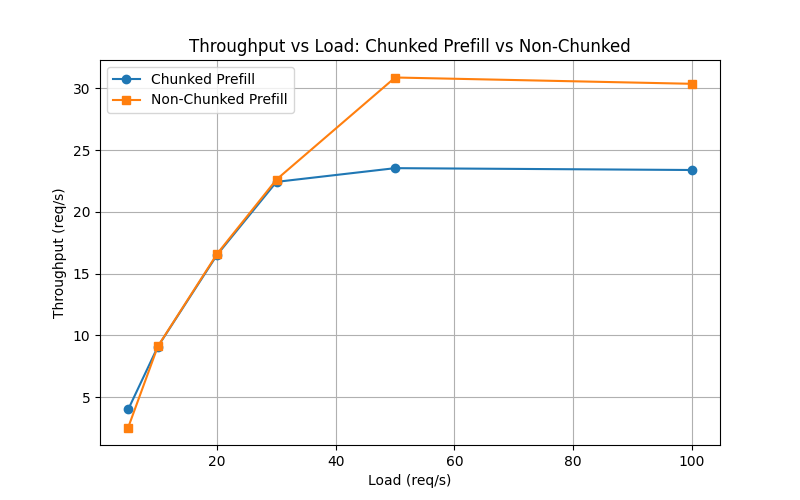
\includegraphics[width=\textwidth]{../results/throughput_comparison_vllm.png}
        \captionof{figure}{Throughput vs Load}
    \end{column}
    \begin{column}{0.4\textwidth}
        \begin{itemize}
            \item Varying the input load, and comparing different modes.
            \item Chunked prefill: limited benefit for small queries.
            \item Prefix caching: major boost to throughput.
            \item Batch tuning further improves efficiency.
        \end{itemize}
    \end{column}
\end{columns}
\begin{block}{Observation}
    Saturation begins at $\sim$300 req/sec — compute bottleneck.
\end{block}
\end{frame}

\section{GPU Memory Breakdown}

\begin{frame}{GPU Memory Breakdown}
    \begin{table}[h!]
\centering
\begin{tabular}{|c|p{4cm}|}
\hline
\textbf{Component} & \textbf{Memory Occupied} \\
\hline
Weights  & 0.93 GiB \\
\hline
Peak Activation  & 4.07 GiB \\
\hline
Non-Torch  & 0.02 GiB \\
\hline
CUDA Graph & 0.41 GiB \\
\hline
KV Cache: Intersection (Prefix)  & 1,280 tokens / 0.0157 GiB \\
\hline
KV Cache: Extras for Requests  & 640 tokens (10 requests × 64 tokens) / 0.0078 GiB \\
\hline
KV Cache: Free & 2,672,880 tokens / 32.8445 GiB \\
\hline
\end{tabular}
\caption{GPU Memory Breakdown and KV Cache Usage}
\label{tab:gpu_memory_breakdown}
\end{table}
\end{frame}

\begin{frame}{Observation: Memory Profiling}
\begin{itemize}
    \item KV Cache footprint is tiny — prefix reuse highly memory-efficient.
    \item Most GPU memory remains free → headroom for larger batches.
    \item Suggests potential for multi-family prefix caching in future work.
\end{itemize}
\end{frame}

\section{Broader Goal}

\begin{frame}{Broader Goal: Motivation}
\begin{itemize}
    \item \textbf{Without prefix sharing:} batch limited by model context length (e.g., 32,768 tokens for a small Qwen model $\rightarrow$ 1500 tokens * 20 requests).
    \item \textbf{With prefix sharing:} utilization-limited, not context-limited. As the number of concurrent requests grows, per-request latency increases, and beyond a point, overall throughput would start declining.
    \begin{block}{Next Step}
    Design a scheduler for families of such requests. At each scheduling step, we must decide whether to prefill a shared prefix or decode tokens for an existing request.
    \end{block}
    \item Explore KV cache offloading to CPU for extended workloads.
\end{itemize}
\end{frame}

\begin{frame}{Future Directions: Quality vs Performance}
\begin{itemize}
    \item Strategy 1: Pass full system prompt each time.
    \item Strategy 2: Fine-tune for families of similar requests.
    \item Study trade-offs:
    \begin{itemize}
        \item \textbf{Performance:} latency, throughput, memory use.
        \item \textbf{Quality:} output accuracy, coherence.
    \end{itemize}
\end{itemize}
\end{frame}

\section{}
\begin{frame}
    \Huge{\centerline{\bf Thank You}}
\end{frame}

\end{document}
